\begin{figure*}[!tbp]
\centering
\begin{subfigure}[b]{0.85\textwidth}
\centering
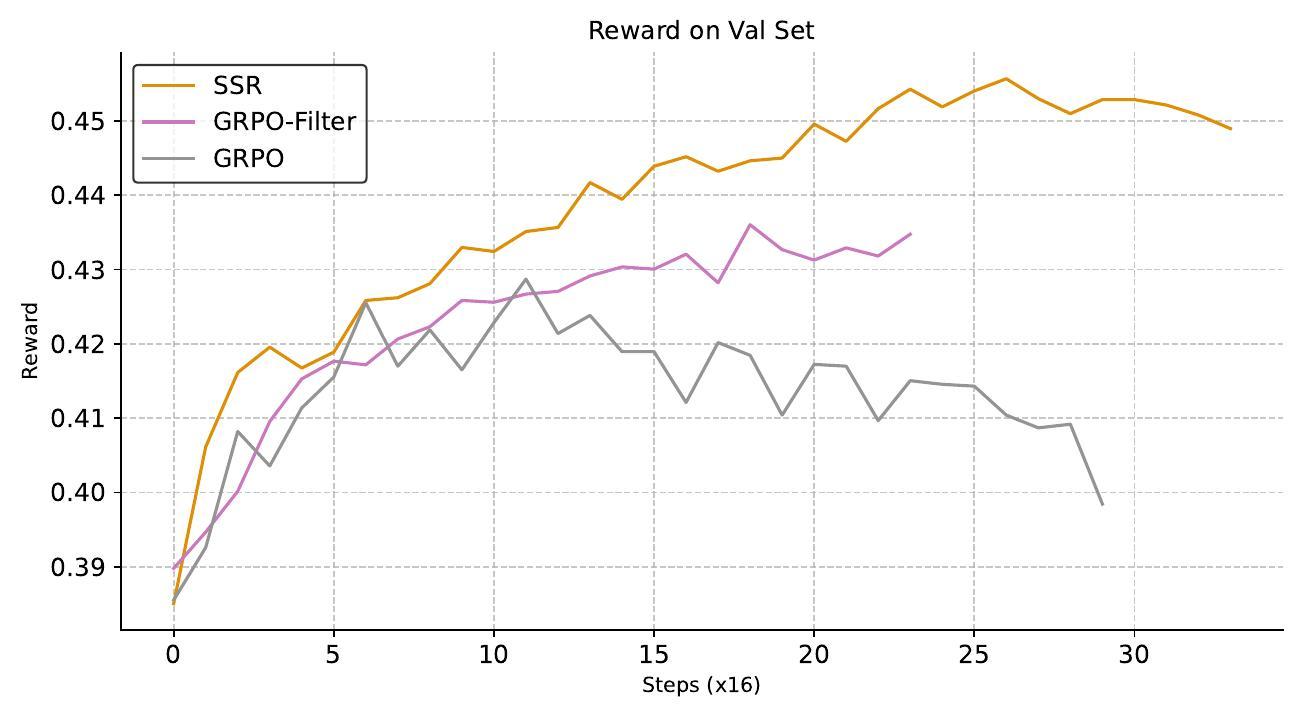
\includegraphics[width=\linewidth]{figures/ssr_eval_curve.jpg}
\caption{Validation reward during training.}
\label{fig:ssr_eval_curve}
\end{subfigure}
\par\smallskip
\begin{subfigure}[b]{\textwidth}
\centering
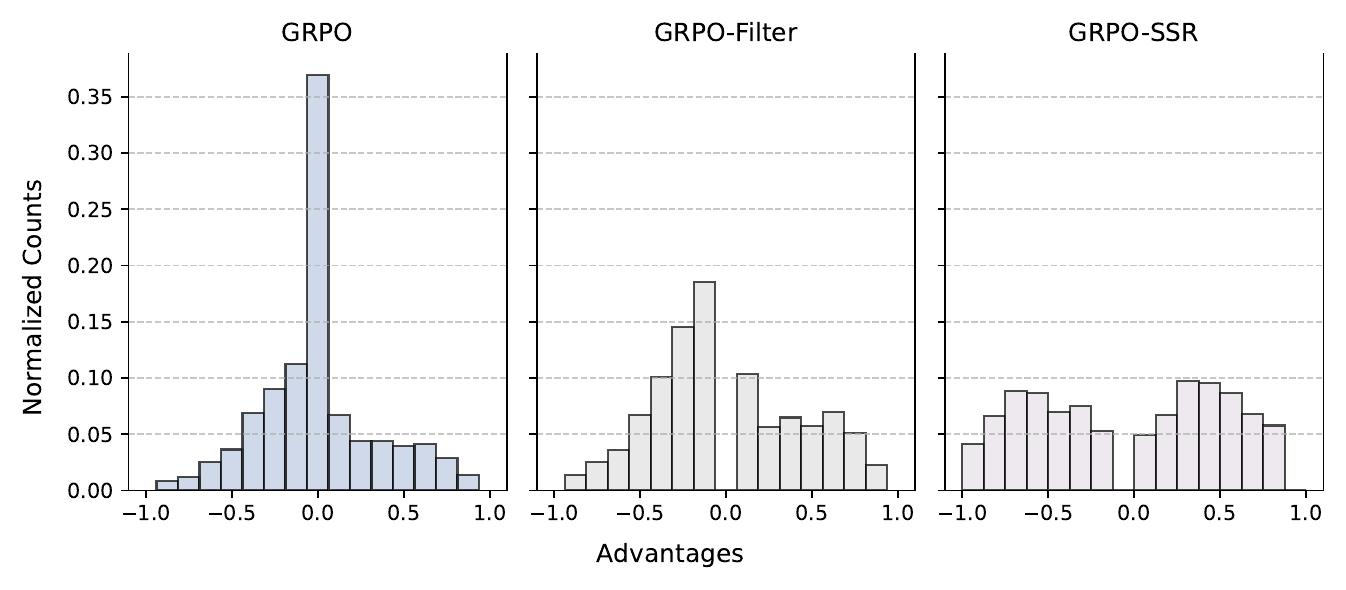
\includegraphics[width=\linewidth]{figures/adv_histogram.jpg}
\caption{Distribution of advantages in training batches.}
\label{fig:adv_histogram}
\end{subfigure}
\caption{\small \textbf{Training dynamics of GRPO, GRPO-Filter and GRPO-SSR.} (a) Mean reward (accuracy) on the held-out validation set; the x-axis counts logged points, one every 16 training steps. Vanilla GRPO peaks at about 0.43 near point 11 ($\approx$180 steps), then declines to about 0.40 by point 29. GRPO-Filter keeps improving to about 0.435 over its shorter run (23 points, $\approx$370 steps). GRPO-SSR improves fastest and reaches about 0.455 around points 23--26 ($\approx$370--420 steps). Each curve is a single run. (b) Normalised histograms of the advantages of the samples used for policy updates. Under GRPO, about 37\% of samples sit in the bin at zero advantage. Filtering removes exact zeros but leaves the mass concentrated at small $|$advantage$|$. SSR's $|$advantage$|$-prioritised replay shifts the mass towards $|$advantage$|\approx 0.3$--$0.9$.}
\label{fig:training_dynamics}
\end{figure*}
